

\documentclass[11pt,a4paper]{article}
\usepackage{hyperref}
\hypersetup{
    colorlinks=true,
    linkcolor=blue,
    filecolor=blue,      
    urlcolor=blue, 
    citecolor=blue
    }

\urlstyle{same}

\usepackage[T1]{fontenc} 
\usepackage[francais]{babel} 
\usepackage[utf8x]{inputenc}
\usepackage{amsmath}
\usepackage{pdfpages}
\usepackage{amsfonts}
\usepackage{amssymb}
\usepackage[margin=1.5cm, top=1cm, bottom=1.5cm]{geometry}
\usepackage{multicol}
\usepackage{graphicx}
\usepackage{calc}
\usepackage{diagbox}
\usepackage{bbold}
\usepackage{array}
\usepackage{minted}
\usepackage{alltt}
\usepackage{amsthm}
\usepackage{forest}
\usepackage{tikz}
\usepackage{enumerate}

\usepackage{float}
\usepackage[caption = false]{subfig}


\usepackage{url}

\usetikzlibrary{automata}
\usetikzlibrary{calc,arrows.meta,positioning}

\title{\textsc{TP n°3 - Support Vector Machine (SVM)}}
\author{Camille MOTTIER}
\date{26 septembre 2024}
% \newcommand{\iddots}{\reflectbox{$\ddots$}}


\usetikzlibrary{arrows.meta}



\setlength{\parindent}{0pt}
\frenchbsetup{StandardLists=true}

\theoremstyle{definition}

\newtheorem{Qu}{Question}


\begin{document}

\maketitle

\



\textbf{\underline{Objectif} : }

\

Le but de ce TP est d'étudier l'utilisation des classifieurs SVM. Nous utiliserons pour cela l'objet \\
\texttt{sklearn.svm.SVC} du package \texttt{scikit-learn}. Nous travaillerons sur deux bases de données : le dataset \texttt{iris} et une base de données composée d'images.

\

Une introduction aux SVM est présente dans le sujet et ne sera pas reprise dans ce compte-rendu. 

\

Certains extraits de code sont cités dans ce rapport, mais le code utilisé pour obtenir les résultats de ce TP est disponible dans son entièreté sur \url{https://github.com/cmottier/TP3_Apprentissage_stat}.

\

\section{Mise en œuvre sur le dataset \texttt{iris}}

Dans cette partie nous utilisons le dataset \texttt{iris} et nous souhaitons classifier la classe 1 contre la classe 2 en utilisant les deux premières variables. Les données sont représentées sur la figure \ref{iris}. Le jeu de données est séparé en données d'apprentissage et en données de test. Voici les instructions utilisées pour cela :

\begin{minted}[bgcolor=gray!8]{python}
# import iris dataset
iris = datasets.load_iris()
X = iris.data
X = scaler.fit_transform(X)
y = iris.target
X = X[y != 0, :2]
y = y[y != 0]

# split train test
X, y = shuffle(X, y)
X_train, X_test, y_train, y_test = train_test_split(X, y, test_size=0.5)
\end{minted}

\begin{figure}[h!]\centering
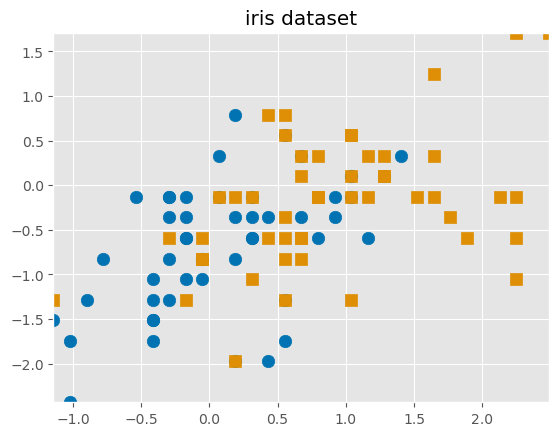
\includegraphics[width=6cm]{Images/iris.png}
\caption{Classes 1 et 2 du dataset \texttt{iris} en fonction des deux premières variables}
\label{iris}
\end{figure}

\

\begin{Qu}~\\

 Nous construisons dans cette question un classifieur SVM à noyau linéaire. 

\begin{minted}[bgcolor=gray!8]{python}
# fit the model with linear kernel
clf_lin = SVC(kernel='linear')
clf_lin.fit(X_train, y_train)

# score
print('Generalization score for linear kernel: %s, %s' %
      (clf_lin.score(X_train, y_train),
       clf_lin.score(X_test, y_test)))
\end{minted}

L'utilisation de ce noyau donne les scores sur les données d'apprentissage et de test suivants :

\

\texttt{Generalization score for linear kernel: 0.74, 0.68}

\

La figure \ref{qu1} représente le classifieur obtenu par cette méthode.

\begin{figure}[h!]\centering
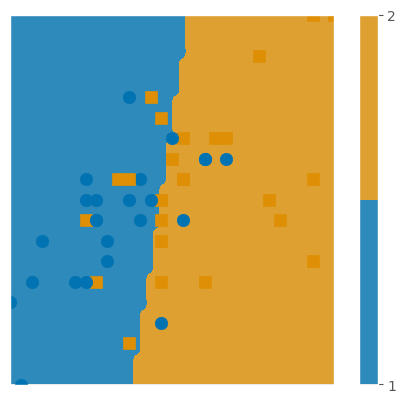
\includegraphics[width=4cm]{Images/qu1.png}
\caption{Classifieur SVM à noyau linéaire et données d'apprentissage du dataset \texttt{iris}}
\label{qu1}
\end{figure}


\end{Qu}

\

\begin{Qu}~\\

Nous souhaitons ici voir si l'emploi d'un noyau polynomial nous permet d'obtenir un meilleur classifieur que celui obtenu précédemment. Après avoir adapté le code précédent, nous obtenons la sortie suivante :

\

\texttt{Generalization score for polynomial kernel: 0.68, 0.52 }

\

La figure \ref{qu2} représente le classifieur obtenu avec le noyau polynomial.

\begin{figure}[h!]\centering
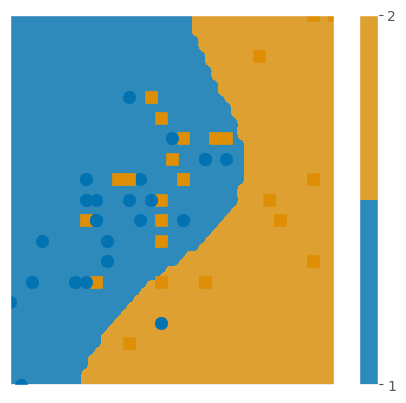
\includegraphics[width=4cm]{Images/qu2.png}
\caption{Classifieur SVM à noyau polynomial et données d'apprentissage du dataset \texttt{iris}}
\label{qu2}
\end{figure}


Nous constatons que le score obtenu avec un noyau polynomial est plus faible que celui obtenu avec un noyau linéaire. Nous préférerons donc le classifieur à noyau linéaire, qui est aussi plus parcimonieux. \\
 La figure \ref{comp} permet de visualiser  les deux classifieurs sur l'ensemble des données du dataset \texttt{iris}. 
 
\begin{figure}[h!]\centering
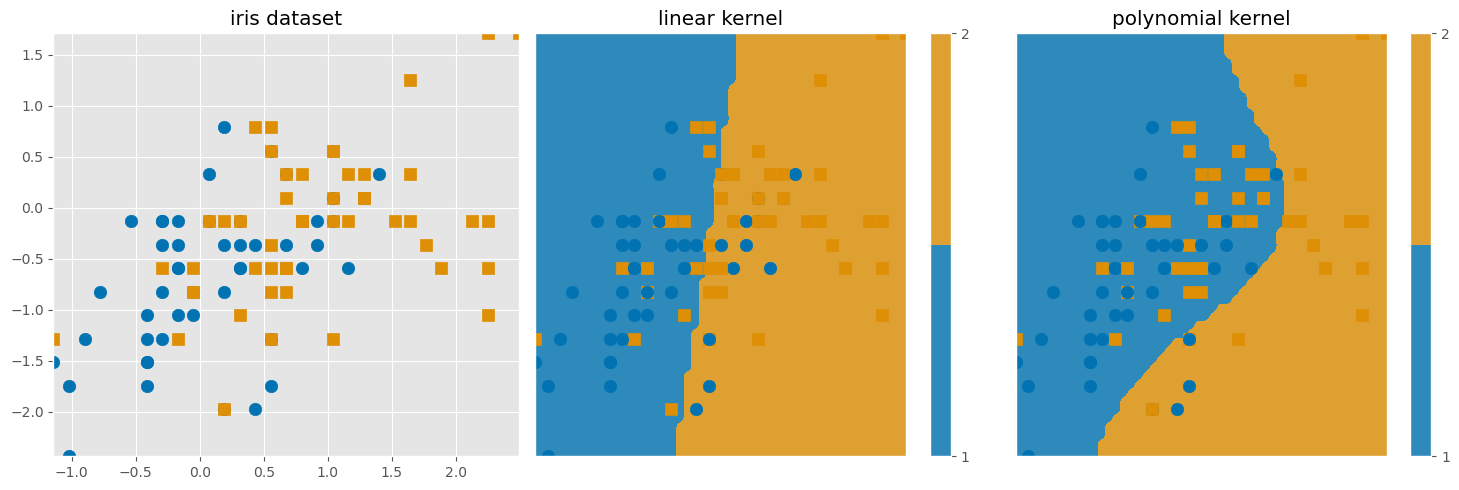
\includegraphics[width=16cm]{Images/comparaison.png}
\caption{Classifieurs SVM à noyaux linéaire et polynomial et dataset \texttt{iris} (apprentissage et test)}
\label{comp}
\end{figure}
 
\end{Qu}

\

\textbf{Remarque.}\\

Notons que les classifieurs construits aux questions 2 et 3 utilisent les paramètres par défaut de la fonction \texttt{sklearn.svm.SVC}. En particulier, la constante de régularisation $C$ est fixée à 1 et  le degré du noyau polynomial est fixé à 3.  En utilisant la fonction \texttt{GridSearchCV}, nous pouvons faire évoluer ces coefficients pour garder le modèle donnant le meilleur score. \\
Dans le cas du noyau linéaire, en considérant pour $C$ des valeurs de $[10^{-3},10^{3}]$ (\texttt{np.logspace(-3, 3, 300)}), nous obtenons les sorties suivantes :

\

\texttt{\{'C': 3.4022997656780714, 'kernel': 'linear'\}}\\
\texttt{Best score : 0.68}\\

Le score sur les données de test est le même que celui obtenu à la question 1, malgré une constante $C$ modifiée. Nous n'améliorons donc pas le classifieur à noyau linéaire.\\
Dans le cas du noyau polynomial, en considérant des degrés entre 1 et 3 et pour $C$ des valeurs de $[10^{-3},10^{3}]$ (\texttt{np.logspace(-3, 3, 5)}), nous obtenons les sorties suivantes :

\

\texttt{\{'C': 1.0, 'degree': 1, 'gamma': 10.0, 'kernel': 'poly'\}}\\
\texttt{Best score : 0.7}\\

Le score sur les données de test est nettement meilleur que celui obtenu à la question 2. Remarquons cependant que le noyau considéré est de degré 1, ce qui correspond à un noyau linéaire. Nous trouvons alors un score et un classifieur très proches de ceux obtenus dans la question 1 (voir la figure \ref{remarque}). \\
En conclusion, nous confirmons avec cette remarque le choix d'un noyau linéaire pour construire le classifieur sur les données du dataset \texttt{iris}.

 
\begin{figure}[h!]\centering
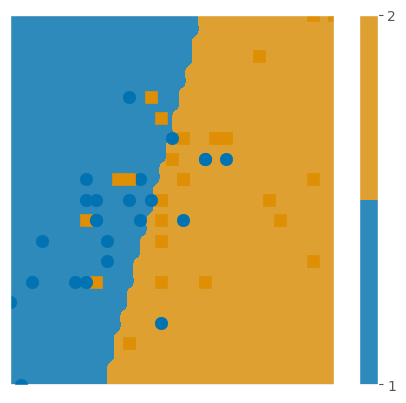
\includegraphics[width=4cm]{Images/rem.png}
\caption{Classifieurs SVM à noyaux polynomial obtenu par  \texttt{GridSearchCV} (sélectionnant un degré 1) et données d'apprentissage du dataset \texttt{iris}}
\label{remarque}
\end{figure}

\section{SVM GUI}

\begin{Qu}~\\

Nous utilisons dans cette question le script \texttt{svm\_gui.py}, disponible à l'adresse : \url{https://scikit-learn.org/1.2/auto_
examples/applications/svm_gui.html}.\\
Il nous permet de visualiser l'impact du choix du paramètre de régularisation $C$. Sur l'exemple testé (voir figure \ref{GUI}), nous pouvons observer que plus $C$ est petit, plus les marges sont grandes, c'est-à-dire qu'on s'autorise plus d'erreurs. On peut constater que sur la dernière figure, tous les points noirs sont mal classés. Ceci vient vraisemblablement du fait qu'il y a un déséquilibre entre le nombre de points noirs et le nombre de points rouges (les points noirs ont un poids négligeable par rapport à celui des points rouges). 

\begin{figure}[h!]\centering
\subfloat[$C=1$]{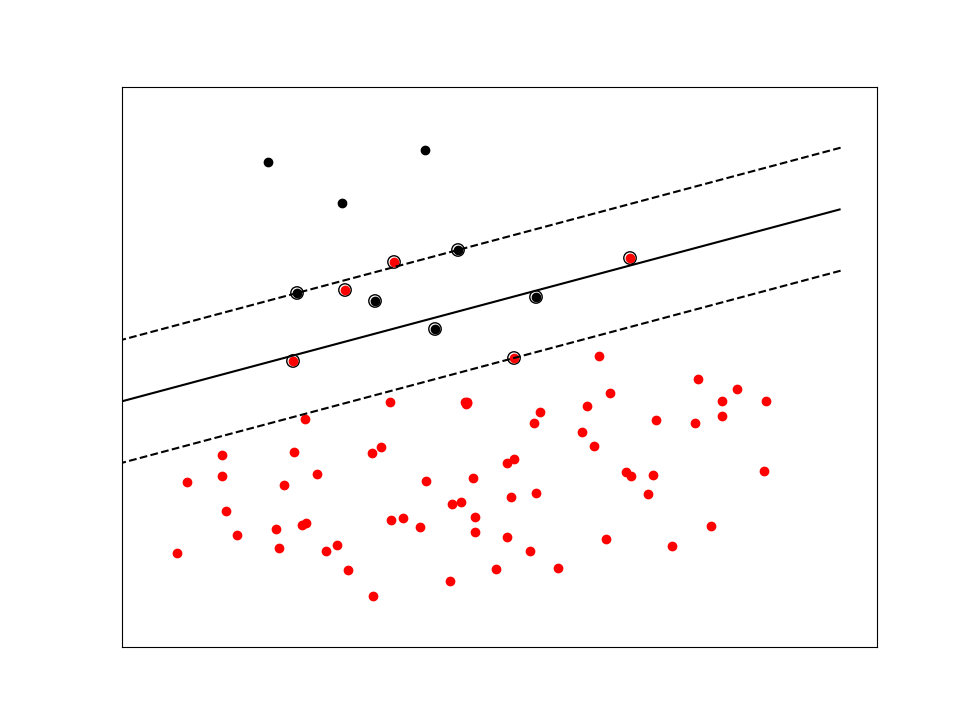
\includegraphics[width=6cm]{Images/GUI1.png}}
\subfloat[$C=0.01$]{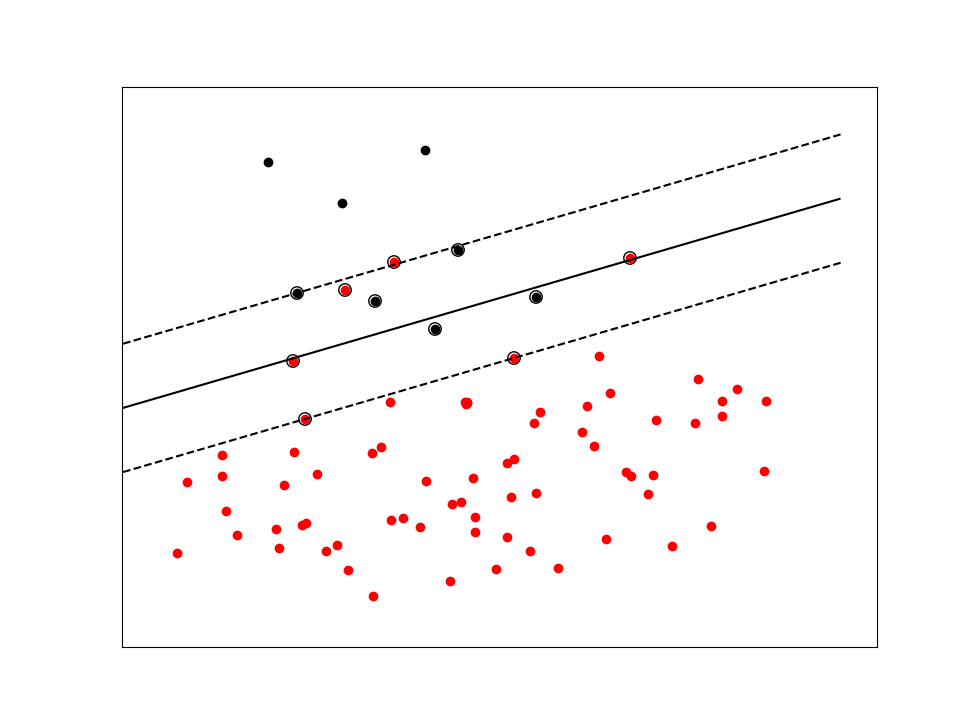
\includegraphics[width=6cm]{Images/GUI2.png}}
\subfloat[$C=0.001$]{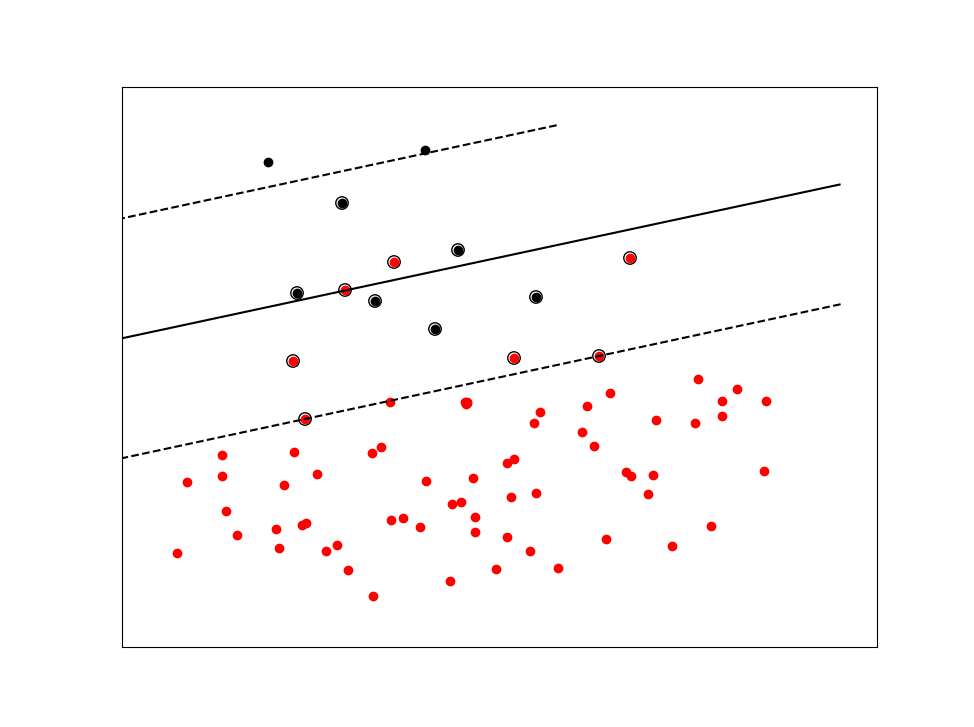
\includegraphics[width=6cm]{Images/GUI3.png}}\\
\subfloat[$C=0.0005$]{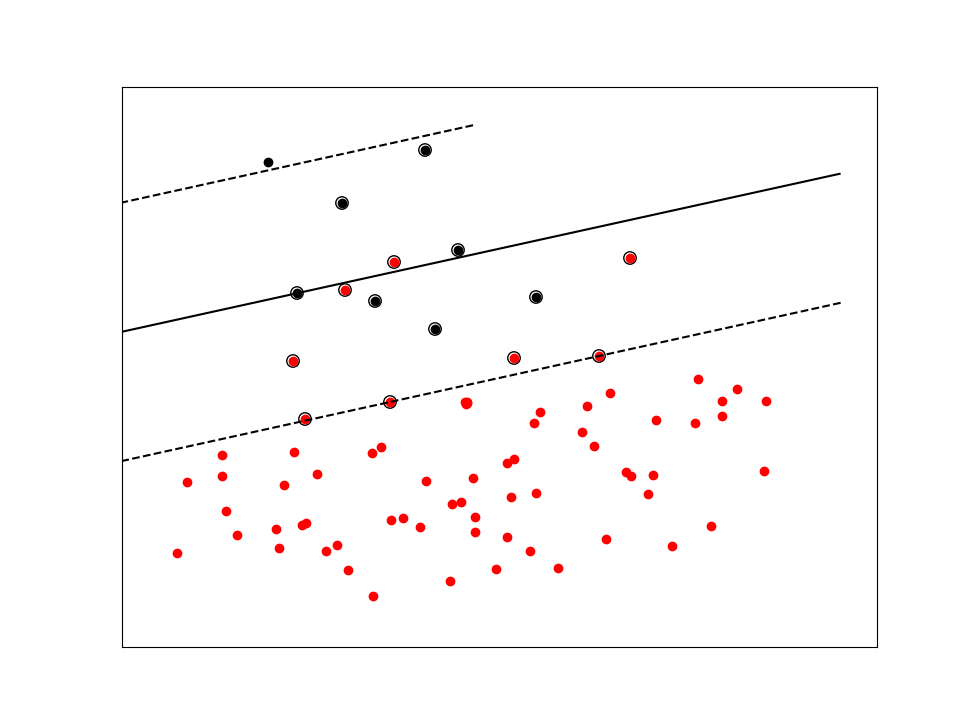
\includegraphics[width=6cm]{Images/GUI4.png}}
\subfloat[$C=0.0001$]{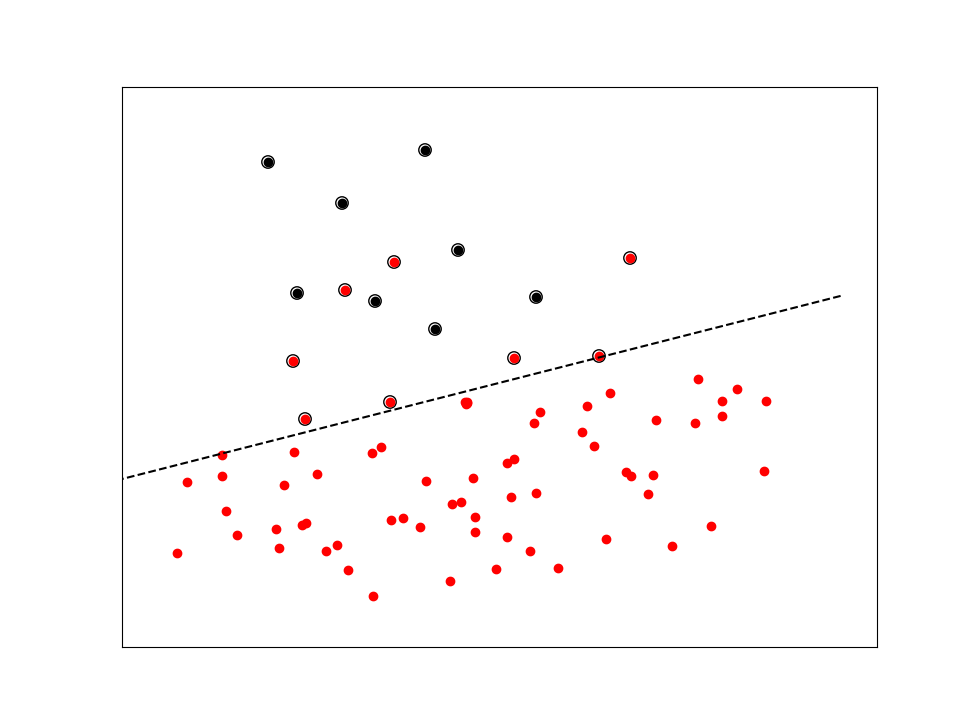
\includegraphics[width=6cm]{Images/GUI5.png}}
\caption{Classifieurs fournis par \texttt{svm\_gui.py} sur un jeu de données ``jouet'', en fonction du paramètre de régularisation $C$}
\label{GUI}
\end{figure}

\end{Qu}

\section{Classification de visages}

Dans cette partie, nous exploitons une base d'images disponible à l'adresse suivante : \url{http://vis-www.cs.umass.edu/lfw/lfw-funneled.tgz}. Nous souhaitons classifier à l'aide d'un SVM à noyau linéaire deux types d'images : celles de Tony Blair et celles de Colin Powell. Nous extrayons donc de la base de données les images les concernant et nous séparons nos données en un jeu d'apprentissage et un jeu de test. 


\

\begin{Qu}~\\

Nous souhaitons observer l'influence du paramètre de régularisation $C$ sur la qualité du classifieur. Pour cela, nous construisons une grille de classifieurs pour des valeurs $C=10^{k}$, $k\in\{-5,\ldots,6\}$ et observons l'erreur de prédiction en fonction de $C$. 

\begin{minted}[bgcolor=gray!8]{python}
# fit a classifier (linear) and test all the Cs
Cs = 10. ** np.arange(-5, 6)
error = []
for C in Cs:
    clf = SVC(kernel='linear', C=C)
    clf.fit(X_train, y_train)
    error.append(1-clf.score(X_test, y_test))
\end{minted}

La figure \ref{qu4} représente les résultats obtenus.


 
\begin{figure}[h!]\centering
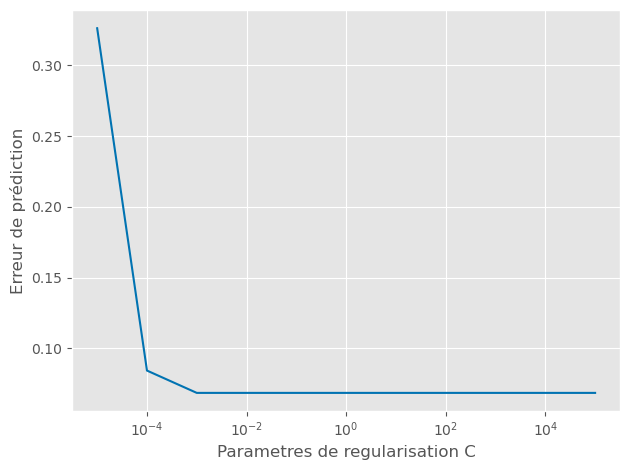
\includegraphics[width=10cm]{Images/erreur.png}
\caption{Erreur de prédiction en fonction du paramètre de régularisation pour des classifieurs SVM à noyau linéaire, sur une base de donnée d'images}
\label{qu4}
\end{figure}

Nous constatons que l'erreur est élevée lorsque $C$ est très petit ($10^{-5}$), diminue jusqu'à $C=10^{-3}$ puis est constante minimale.
Ce résultat est cohérent car lorsque $C$ est trop petit, nous ne pénalisons que très peu les mauvais classements, donc ceux-ci peuvent être nombreux. \\
Nous obtenons pour $C=10^{-3}$ :  

\begin{verbatim}
Best C: 0.001
Best accuracy: 0.9315789473684211
Predicting the people names on the testing set
Chance level : 0.6210526315789474
\end{verbatim}


Le score est élevé, en comparaison à celui obtenu en prédisant toujours la classe majoritaire. Ainsi, on peut dire que le classifieur optimal est de bonne qualité. La figure \ref{blair} illustre les résultats donnés par la prédiction sur un certain nombre d'images.

 
\begin{figure}[h!]\centering
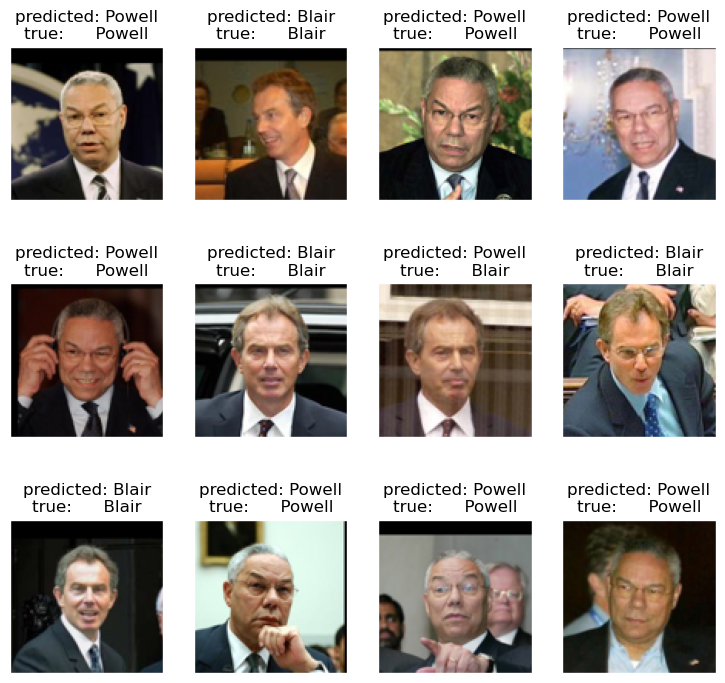
\includegraphics[width=12cm]{Images/blair.png}
\caption{Prédictions faites par le classificateur optimal sur un échantillon d'images}
\label{blair}
\end{figure}

Nous pouvons aussi observer quels sont les pixels (ie les variables) qui ont joué un rôle prépondérant, en visualisant les poids qui leur ont été associé. C'est ce que montre la figure \ref{pixel}. Nous devinons l'importance des cheveux, des sourcils et de la bouche pour la prédiction.

 
\begin{figure}[h!]\centering
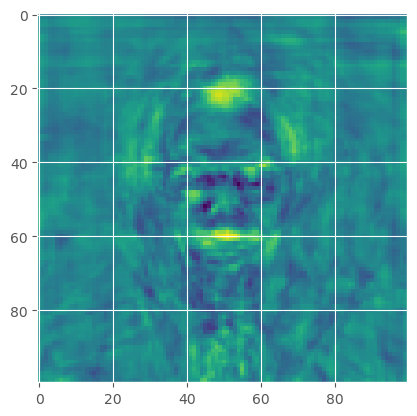
\includegraphics[width=5cm]{Images/pixel.png}
\caption{Poids des différentes variables dans le classifieur optimal obtenu}
\label{pixel}
\end{figure}

\end{Qu}

\

\begin{Qu}~\\

Montrons que le score de prédiction est sensible au bruit. Pour cela, nous ajoutons des variables de bruit et recommençons la prédiction. 
Nous considérons donc le code suivant : 

\begin{minted}[bgcolor=gray!8]{python}
# Ajout des variables de nuisances
sigma = 1
noise = sigma * np.random.randn(n_samples, 300, )
X_noisy = np.concatenate((X, noise), axis=1)
X_noisy = X_noisy[:,np.random.permutation(X_noisy.shape[1])] # correction du code fourni
run_svm_cv(X_noisy,y)
\end{minted}

Le bruitage consiste à ajouter 300 variables (pixels) de bruit, suivant une loi normale centrée réduite, et à les mélanger aux autres. Nous obtenons alors les valeurs suivantes avec et sans nuisances :

\begin{verbatim}
Score sans variable de nuisance
Generalization score for linear kernel: 1.0, 0.9315789473684211

Score avec variable de nuisance
Generalization score for linear kernel: 1.0, 0.9105263157894737
\end{verbatim}


Nous constatons alors que, malgré les variables de bruit ajoutées, le classifieur est toujours d'excellente qualité. On peut supposer que cela vient du fait que nous avons ajouté seulement 300 variables de bruit, avec un écart-type de 1, à 10000 déjà existantes. 
En bruitant cette fois-ci avec 1000 variables supplémentaires d'écart-type égal à 5, nous voyons se dessiner une baisse de performance :

\begin{verbatim}
Score avec variable de nuisance
Generalization score for linear kernel: 1.0, 0.7473684210526316 
\end{verbatim}

Il serait peut-être intéressant de chercher à bruiter les variables ayant un poids fort dans la prédiction afin de visualiser l'effet d'un bruit sur ces variables. La performance devrait alors chuter davantage. 



\end{Qu}

\

\begin{Qu}~\\

Nous cherchons à améliorer la prédiction obtenue dans la question précédente à l'aide d'une réduction de dimension par analyse à composante principale. Voici le code utilisé pour cela : 

\begin{minted}[bgcolor=gray!8]{python}
# Scale features
X_noisy -= np.mean(X_noisy, axis=0)
X_noisy /= np.std(X_noisy, axis=0)

# PCA
n_components = 50
X_pca = PCA(n_components=n_components).fit_transform(X_noisy)

print("Score apres reduction de dimension")
run_svm_cv(X_pca,y)
\end{minted}

Nous obtenons alors : 

\begin{verbatim}
Score apres reduction de dimension
Generalization score for linear kernel: 0.9526315789473684, 0.868421052631579
\end{verbatim}

Nous remarquons que le score obtenu après l'ACP est meilleur que celui obtenu avec les variables bruitées, car les directions de bruit ont été supprimées en sélectionnant 50 composantes. Notons qu'en augmentant le nombre de composantes, le score obtenu reste similaire. Il faudrait observer ce qu'il se passe en diminuant le nombre de composantes, mais ma machine n'arrive pas au bout des calculs dans ces cas là. 


 
\end{Qu}







\end{document}

